\section{Data Analysis}
\label{data_analysis}
Following Section \ref{data_collection}, there are now three different datasets. It is now time to visualise and analyse the data in order to gain insights before using it in order to train an AI. This section describes the method used and the results for each dataset.

\subsection{Method}
In the frist place, we worked in a Python Notebook which allows us to execute code cells independantly making the analysis process more user-friendly.\\
Acceleration and GPS (if available) data are loaded in Pandas dataframes giving access to many usefull functions to understand the data. The most important methods are \textsf{describe} and \textsf{isna}. The first one provides general statistic values regarding the data (count, mean, standard deviation...) and the second one can be used with \textsf{sum} in order to compute the amount of missing values for each attribute.\\
Finally, different methods allowing to visualise accelerometric and/or GPS data were implemented. Eventhough Matplotlib figures are great (Figure \ref{bump_1}), HTML figures created with Plotly have the huge advantage of being interactive on all devices and operating systems with a internet browser. This means it is possible to zoom in and out on a specific part of a graph which is very important when working with high frequencies or long recordings. Two types of graphs look interesting depending of the need:
\begin{itemize}
    \item Every attributes on a single graph (Figure \ref{bump_2})
    \item Each attribute on a separate graph (Figure \ref{bump_3})
\end{itemize}
Working with HTML figures also allows to tie acceleration and GPS data on a single page (Figure \ref{gps_1}).\\

In a second time, we created a Python script which automaticaly generates figures depending of the type of data and user preferences (output format) specified in arguments.\\

\subsection{Robot}

\noindent
\begin{minipage}[!hc]{0.12\textwidth}
   \textbf{Reminder}
\end{minipage}
\vrule\enskip\vrule\quad\begin{minipage}{\dimexpr 0.87\textwidth-0.8pt-1.5em}
The force of gravity has been removed from the acceleration measurements and the Arduino device was mounted on the robot taking care of the orientation of the IMU:
\begin{itemize}
    \item Positive X = Froward
    \item Positive Y = Left
    \item Positive Z = Up
\end{itemize}
\end{minipage}
\\
As expected, there is no missing values in the data recorded with the Arduino device and, on the most simple samples, it is really easy to understand the acceleration data. On Figure \ref{bump_1}, we can clearly see huge variations along the Z axis when passing the bump (meaning the vehicle is effectively changing speed along verticaly due to the bump) and smaller variations along the X axis (because the vehicle is slowed down on the rising section and accelerates when going down). We can also see some even smaller variations form side to side (Y axis) which are mostlikely due to the robot damping system and vibrations of the mounting plate.\\

\noindent
\begin{minipage}[!hc]{0.12\textwidth}
   \textbf{Remark}
\end{minipage}
\vrule\enskip\vrule\quad\begin{minipage}{\dimexpr 0.87\textwidth-0.8pt-1.5em}
The sampling frequency (i.e. horizontal granularity) is defined by the Arduino program as: \(f = \frac{1}{10^{-3}}\) which correspond to a delay of 10 ms between two measures.\\
It is important to pay attention to the vertical scale of each graph.
\end{minipage}

\begin{figure}
    \center
    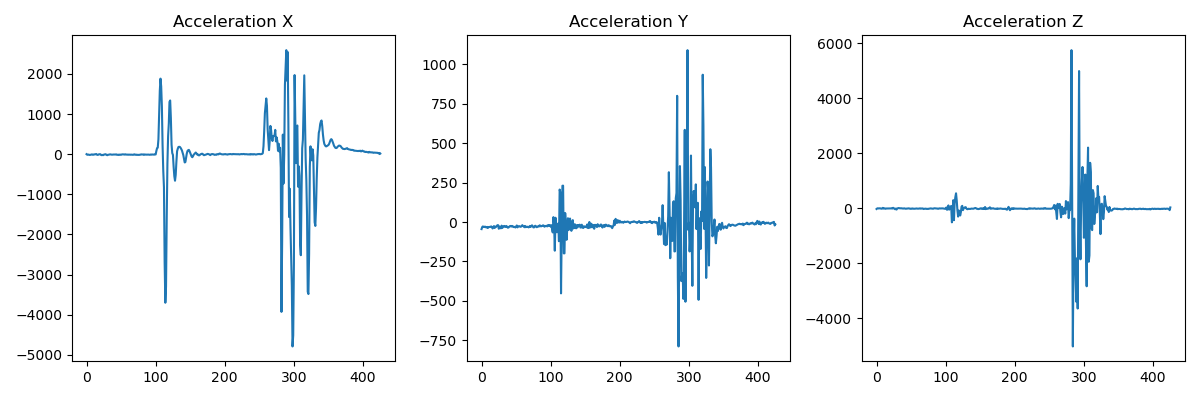
\includegraphics[scale=0.5]{img/DATA1.png}
    \caption{Acceleration data recorded with the Arduino device on the robot while rolling straight on a small speed-bump (plotted with Matplotlib)}
    \label{bump_1}
\end{figure}

Plotting data on a single graph is usefull in order to check the timing of shocks along the three axis. Figure \ref{bump_2} shows there are acceleration variations during two brief periods regardless of the axis. These periods correspond to the start of the vehicle (when it begins to move, ranging from 100 to 150) and the ride over the bump (starting at 250).\\

\begin{figure}
    \center
    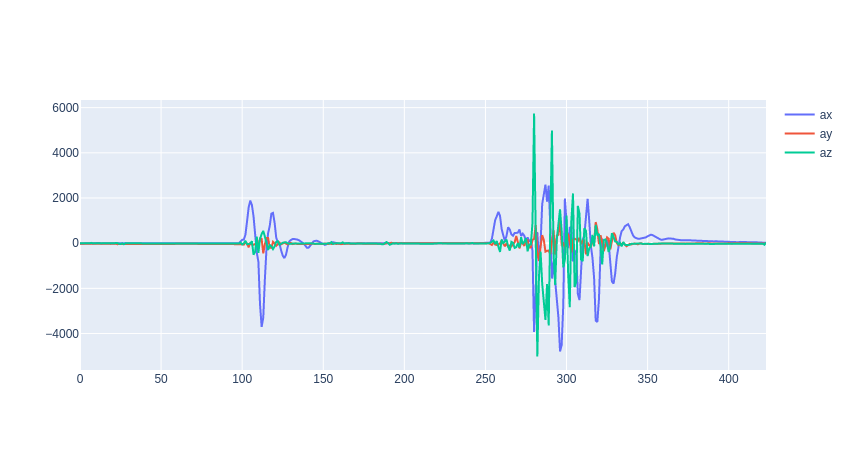
\includegraphics[scale=.5]{img/DATA1_combined.png}
    \caption{Acceleration data recorded with the Arduino device on the robot while rolling straight on a small speed-bump (plotted with Plotly)}
    \label{bump_2}
\end{figure}

However looking at longer recordings, it is already difficult to recognize obstacles at a glance. Figure \ref{bump_3} correspond to the robot rolling in a hole, then over a small crack and finally on top of some little bumps. This recording only lasts a couple of seconds so it is way shorter than the data we expect to get when collecting data on real journeys.\\

\begin{figure}
    \center
    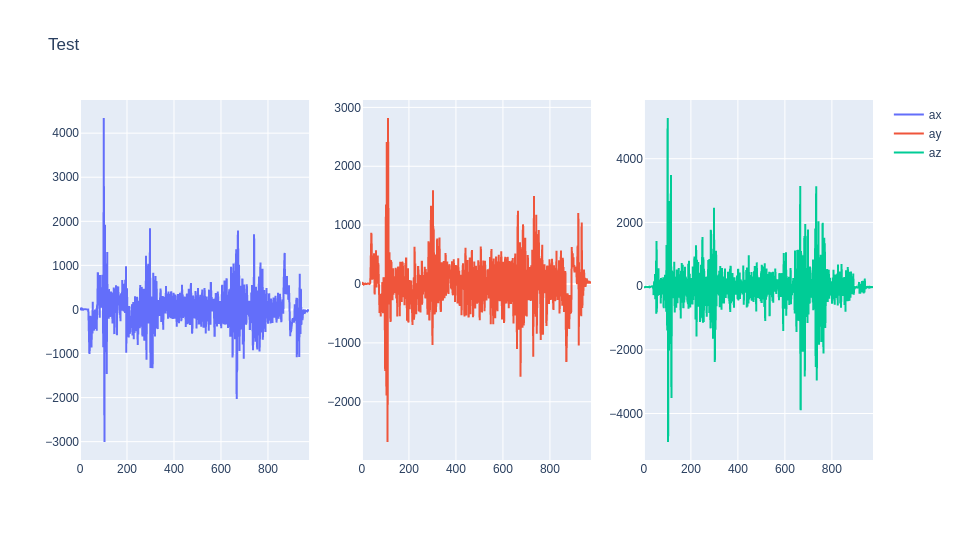
\includegraphics[scale=.5]{img/DATA9.png}
    \caption{Acceleration data recorded with the Arduino device on the robot while rolling on various obstacles (plotted with Plotly)}
    \label{bump_3}
\end{figure}

\subsection{Car}
The data collected in a car was also analysed using the same method and fortunatly there was no missing values to report. However we noticed small fluctuations in the sampling rate. The timestamps on the acceleration data are separated by values ranging from 20 to 30 milliseconds. This issue has not been adressed yet but it is only a minor correction and it does not prevents us from visualising GPS data and making sure we can access accelerometric data.\\

It seems that the recording method needs to be improved. On the one hand, GPS data are correct and quite precise, but on the other hand, acceleration data has an unexpected and incoherent shape (Figure \ref{gps_1}).\\

\begin{figure}
    \center
    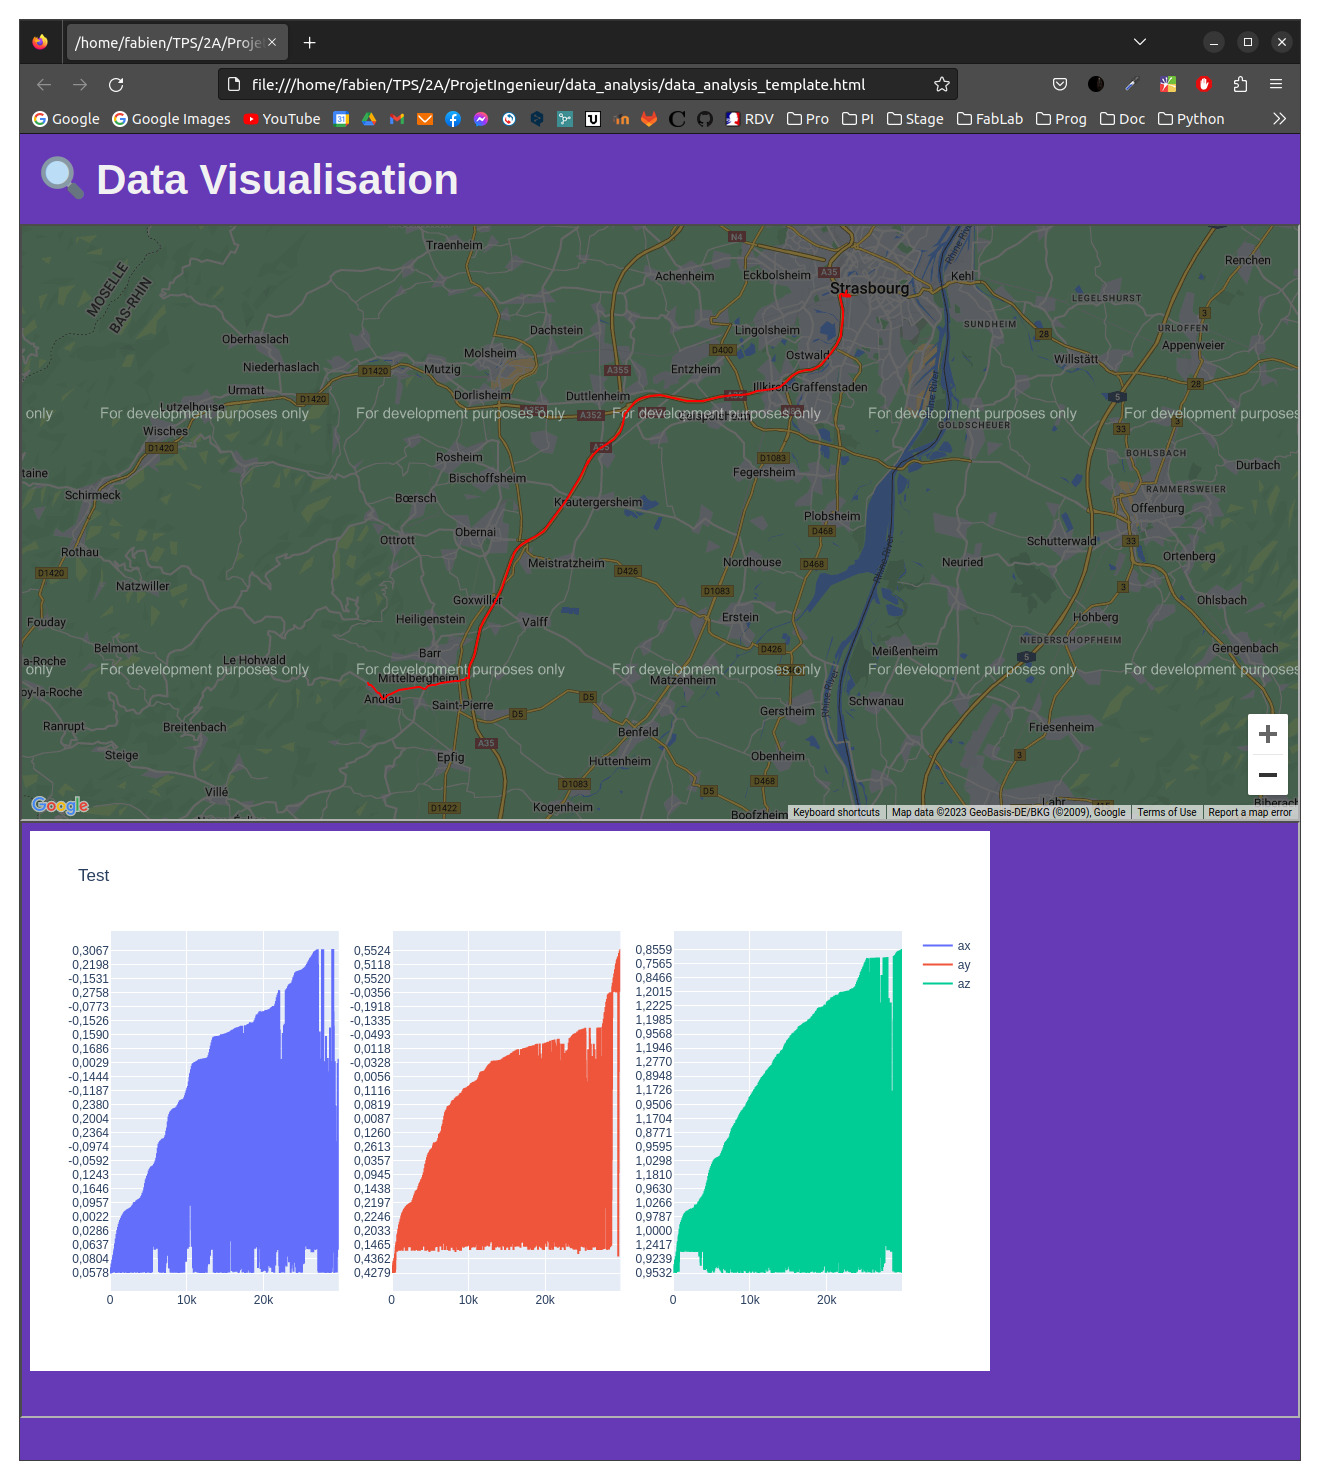
\includegraphics[scale=.25]{img/gps_1.png}
    \caption{Acceleration and GPS data recorded with a smartphone and a smartwatch in a car (plotted with Plotly and Gmplot)}
    \label{gps_1}
\end{figure}

\subsection{Online Dataset}
The data contained in this last dataset requires a different processing. Eventhough its origin and the methodology used to build it are still unknown, we managed to get a few informations from the files.\\
First and formost these files contain labelised data: most files are \textsf{json} files containing acceleration along the X, Y and Z axis as well as some metadata at the beginning. This metadata contains among other things the time period of the vehicle riding on the obstacle and the type of obstalce (for the most part \textit{Metal bumps}).\\
It is also worth mentioning that the files are separated in folders according to the speed (either 30 or 50 of an undetermined unit) and their use (training or testing).\\

An included Python script allowed us to visualise some recordings (Figure \ref{online_bumps}). According to a couple of previews, metadata looks correct but we will have to investigate and find more information about this dataset.\\

\begin{figure}
    \center
    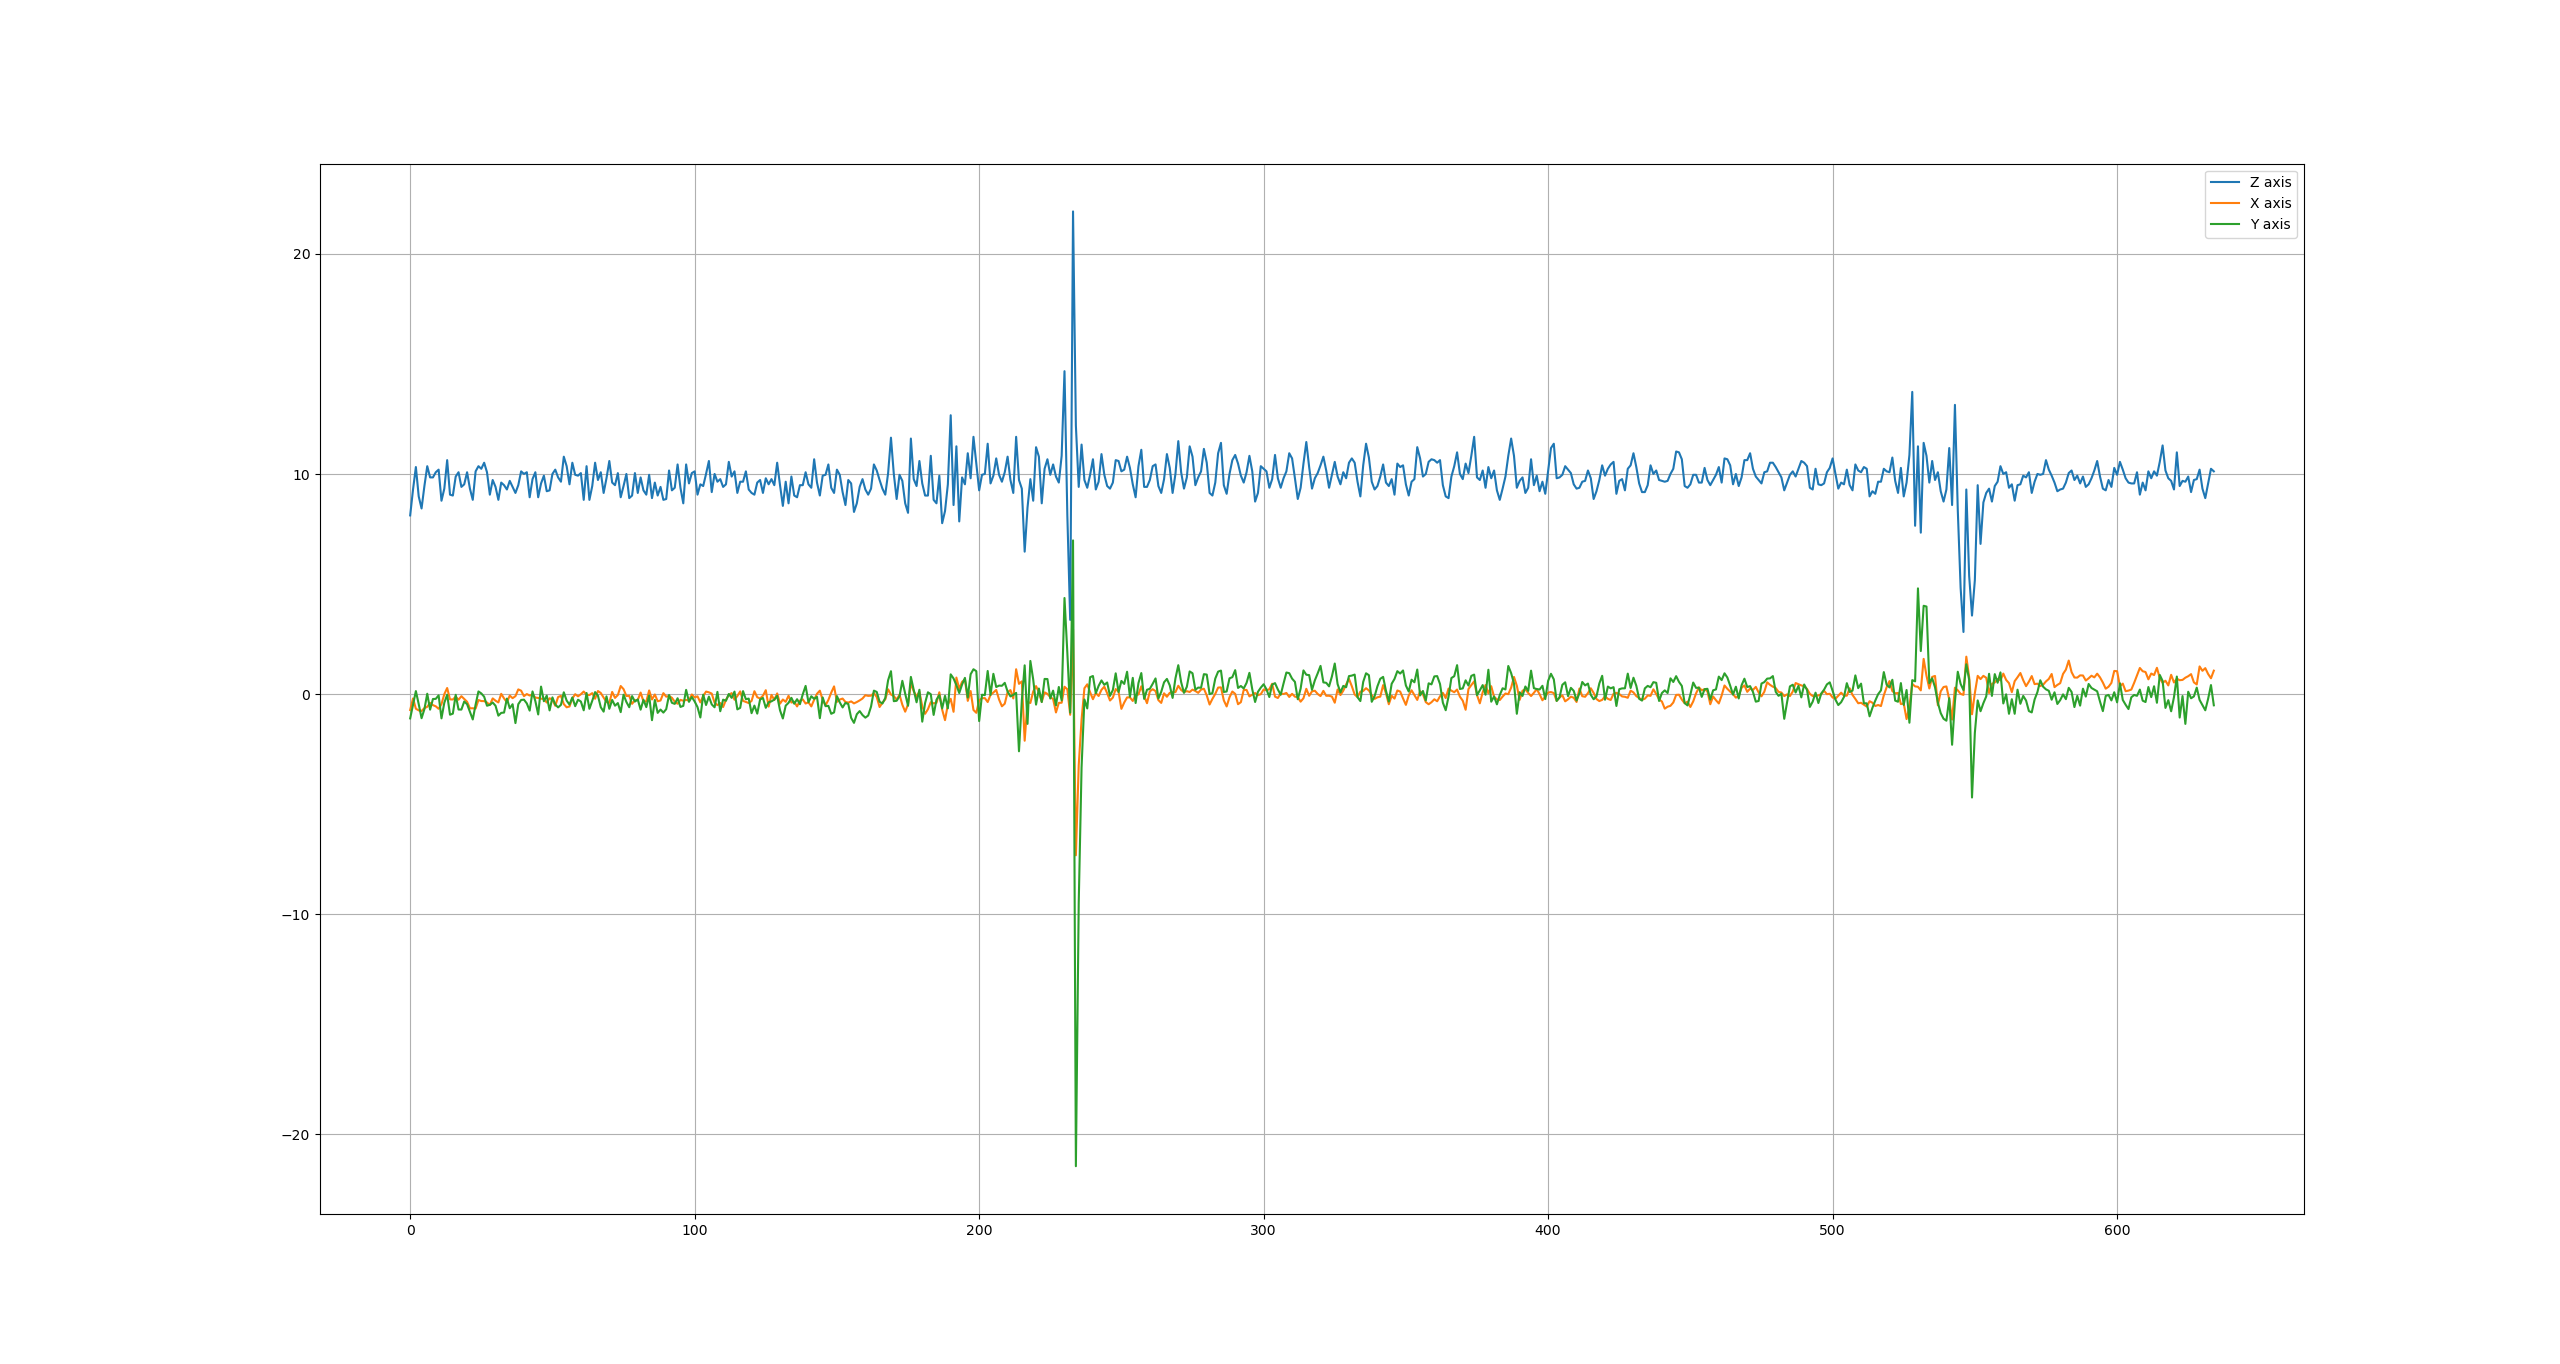
\includegraphics[scale=.25]{img/online_bumps.png}
    \caption{Acceleration data from a mysterious dataset}
    \label{online_bumps}
\end{figure}

\noindent
\begin{minipage}[!hc]{0.12\textwidth}
   \textbf{Remark}
\end{minipage}
\vrule\enskip\vrule\quad\begin{minipage}{\dimexpr 0.87\textwidth-0.8pt-1.5em}
This dataset does not reduce the force of gravity from the acceleration which explains the close-to-ten offset of the Z component.
\end{minipage}